\documentclass[conference]{IEEEtran}
\IEEEoverridecommandlockouts
% The preceding line is only needed to identify funding in the first footnote. If that is unneeded, please comment it out.
\usepackage{amsmath,amssymb,amsfonts}
\usepackage{algorithmic}
\usepackage{graphicx}
\usepackage{textcomp}
\usepackage{xcolor}
\usepackage{cite}
\usepackage{url}
\def\BibTeX{{\rm B\kern-.05em{\sc i\kern-.025em b}\kern-.08em
    T\kern-.1667em\lower.7ex\hbox{E}\kern-.125emX}}
\begin{document}

\title{An Open-Source Geospatial Pipeline for Water Distribution Monitoring: Integrating VGI, Automated Prioritization, and Synthetic Data Generation}

\author{\IEEEauthorblockN{João Victor Teófilo Salgado}
\IEEEauthorblockA{\textit{Computer Science Department} \\
\textit{Universidade Federal de Lavras}\\
Lavras, Brasil \\
joao.salgado1@estudante.ufla.br}
\and
\IEEEauthorblockN{Cyntia Virolli Cid Molina}
\IEEEauthorblockA{\textit{GEPIDE - Research Group in Spatial Data Infrastructure (EACH-USP)} \\
\textit{Universidade de São Paulo)}\\
São Paulo, Brasil\\
cid.virolli@gmail.com}
\and
\IEEEauthorblockN{Ogobuchi Daniel Okey}
\IEEEauthorblockA{\textit{Computer Science Department} \\
\textit{Universidade Federal do ABC}\\
São Paulo, Brasil \\
okey.ogobuchi@ufabc.edu.br}
\and
\IEEEauthorblockN{Demostenes Zegarra Rodriguez}
\IEEEauthorblockA{\textit{Computer Science Department} \\
\textit{Universidade Federal de Lavras}\\
Lavras, Brasil \\
demostenes.zegarra@ufla.br}
\and
\IEEEauthorblockN{Renata Lopes Rosa}
\IEEEauthorblockA{\textit{Computer Science Department} \\
\textit{Universidade Federal de Lavras}\\
Lavras, Brasil \\
renata.rosa@ufla.br}
}

\maketitle

\begin{abstract}
Efficient monitoring of water distribution systems is crucial for minimizing water loss and ensuring service continuity. However, small-scale utilities and NGOs often face significant financial and technical barriers when implementing advanced proprietary Geographic Information Systems (GIS). To address this, this paper presents a 100\% open-source, event-driven geospatial architecture designed to ingest, process, and prioritize Volunteered Geographic Information (VGI) in real time. The proposed pipeline decouples field data collection from an automated in-database analytical engine hosted in PostGIS. A novel spatial prioritization algorithm consolidates redundant crowdsourced reports using a Minkowski-based DBSCAN clustering approach and ranks operational urgency via spatial Multi-Criteria Decision Analysis (MCDA). Furthermore, the proposed MCDA model dynamically reallocated critical incidents near essential services to the top of the maintenance queue. To overcome the VGI "cold start" challenge and calibrate clustering parameters, we also introduce a demographic-driven synthetic data generation model utilizing census tracts, building footprints and existing water network data. The results demonstrate that this in-database framework provides a scalable, low-latency, and interoperable solution for smart city management and humanitarian relief efforts.

\end{abstract}

\begin{IEEEkeywords}
open-source software, geospatial data, water monitoring system, data generation, gis, vgi
\end{IEEEkeywords}

\section{Introduction}

\IEEEPARstart{T}he management of Water Distribution Systems (WDS) is a critical challenge for urban infrastructure, directly impacting public health, economic stability, and environmental sustainability. Efficient monitoring of water leaks and supply disruptions is essential to minimize Non-Revenue Water (NRW) and ensure service continuity \cite{liemberger2019}. However, many small-scale water utilities and Non-Governmental Organizations (NGOs) in developing regions face significant barriers to implementing advanced monitoring systems. These barriers often include high licensing costs of proprietary Geographic Information Systems (GIS) \cite{livaja2017geospatial,salgado2024automated} and the technical complexity of integrating real-time field data with legacy infrastructure \cite{coetzee2020}.

In this context, Volunteered Geographic Information (VGI) emerges as a powerful paradigm, transforming citizens into "human sensors" capable of providing timely spatial data on network failures \cite{goodchild2007}. While VGI has been successfully applied in disaster management and urban mapping, its systematic integration into water utility workflows remains limited by the lack of accessible, end-to-end architectures that can prioritize reports and validate system performance before large-scale deployment.

This paper presents a robust, 100\% open-source solution designed to bridge this gap. By integrating KoboToolbox and n8n for automated data ingestion, the architecture leverages PostGIS to host a novel spatial prioritization algorithm. This algorithm acts as the core analytical engine, automatically triaging and ranking VGI reports based on spatial constraints and operational urgency. Furthermore, the system employs QGIS Server to facilitate open data publishing for researchers and the community, while Apache Superset provides Business Intelligence (BI) capabilities for interactive network analysis and decision-making. Thus, the primary contributions of this work are the development of this spatial prioritization algorithm and an innovative methodology for generating organic synthetic incidents, allowing utilities to simulate and optimize response strategies based on demographic and census data.

In this paper, we evaluate the implementation of this open-source ecosystem, focusing heavily on the performance and accuracy of the proposed prioritization algorithm when handling real-world VGI inputs. We describe the technical orchestration between the data collection and the spatial analysis layers, highlighting how small entities can deploy these tools without specialized infrastructure. Additionally, we analyze the algorithm's efficiency and validate the framework's scalability using the synthetic data generation model to reflect realistic urban patterns.

The sections in this document are structured as follows: Section 2 explores the literature regarding VGI and open-source technologies in urban infrastructure. Section 3 details the system's architecture, emphasizing the mathematical and spatial logic behind the prioritization algorithm and the synthetic data generation. Section 4 presents the experimental results and discusses the system's impact on resource allocation. Lastly, Section 5 concludes the work and highlights future directions for open-source utility management.

\section{Related Work}

\subsection{VGI Applications in Smart Cities and Utilities}

The integration of Volunteered Geographic Information (VGI) into urban management has evolved significantly in recent years. In the context of smart cities, contemporary studies highlight VGI and GeoAI as transformative tools for participatory mapping, civic reporting, and enhancing community-driven governance \cite{kumas2025, naghavi2022}. For utility management—specifically within drinking water networks—participatory GIS is increasingly recognized as a vital mechanism for long-term collaboration, particularly in small rural or NGO-operated systems that lack the resources for traditional asset mapping and telemetry \cite{mcdonald2025}. However, despite these methodological advances, the majority of current literature continues to focus heavily on front-end engagement, gamification, and data collection interfaces. Consequently, there remains a noticeable gap regarding the back-end analytical frameworks required to automatically process, validate, and extract actionable operational intelligence from high volumes of crowdsourced utility reports in real time.

\subsection{Open-Source Spatial Data Infrastructures (SDI)}

To process spatial utility data, municipal governments traditionally rely on proprietary Geographic Information Systems (GIS). These systems impose high financial and technical barriers for smaller entities. In response, Open-Source Spatial Data Infrastructures (SDI) have emerged as robust, cost-efficient alternatives. Recent implementations demonstrate that stacks utilizing PostgreSQL/PostGIS for spatial data persistence and QGIS Server for map publishing provide advanced interoperability and spatial analytics that rival proprietary solutions, making them highly suitable for managing complex water supply networks \cite{brovelli2016}. Furthermore, initiatives incorporating open-source hydraulic ecosystems have proven the feasibility of managing the entire lifecycle of water utilities without restrictive licensing \cite{brovelli2016}. Despite these established advantages, few studies document end-to-end architectures that seamlessly integrate automated, event-driven data ingestion for real-time triage of civic reports.

\subsection{Spatial Triage and Incident Prioritization}

The influx of Volunteered Geographic Information inevitably generates challenges related to data redundancy and triage, particularly when multiple citizens report the same visible leak or service interruption. To address spatial redundancy, the literature frequently employs clustering algorithms, such as DBSCAN, or Kernel Density Estimation (KDE) to identify incident hotspots and consolidate duplicate reports \cite{dealbuquerque2015}. Furthermore, to determine the operational urgency of these incidents, recent studies have proposed Multi-Criteria Decision Analysis (MCDA) and network topology assessments. These methods rank the severity of water supply failures based on variables such as proximity to critical infrastructure (e.g., hospitals or schools) and the estimated affected population \cite{zyoud2016}.

While these methodologies are analytically robust, they are predominantly executed as batch post-processing tasks within external desktop GIS environments or middleware scripts (e.g., Python or R). This reliance on external processing layers introduces latency and increases overall system complexity, which is often prohibitive for small utilities and NGOs. Consequently, there is a distinct scarcity of research exploring spatial triage algorithms embedded directly within the Spatial Database Management System (SDBMS) \cite{obe2021}. Executing prioritization logic natively—using automated spatial procedures within environments like PostGIS—immediately upon data ingestion remains a critical gap in achieving real-time, low-infrastructure utility management.

\subsection{Synthetic Data Generation in Geospatial Validation}

The validation of spatial triage algorithms poses a significant methodological challenge, primarily due to the scarcity of open, high-resolution datasets reflecting real-world utility failures. To overcome the lack of accessible data—often restricted by privacy concerns and strict security protocols of utility companies—researchers frequently rely on synthetic spatial data generation \cite{mody2023}. In the context of Volunteered Geographic Information (VGI), this dependency is exacerbated by the "cold start" problem: it is inherently difficult to empirically test the performance of a crowd-sourced reporting architecture before it achieves widespread civic adoption \cite{mazzoleni2019}.

However, a critical limitation in current geospatial validation frameworks is the difficulty of generating synthetic scenarios that accurately mirror reality. The majority of traditional synthetic data generators distribute points either purely randomly across a bounding box or strictly based on the topological geometry of the network \cite{mcalinden2024}. Neither approach accurately reflects the organic nature of VGI. Real-world civic reports of water leaks are not uniformly distributed; rather, they are deeply correlated with underlying urban dynamics, such as population density, infrastructure age, and local socio-economic patterns. Validating an incident prioritization algorithm with uniform or purely random spatial distributions fails to evaluate the system's true capacity to handle the organic clustering and human-driven hotspots typical of civic monitoring \cite{sun2024}. Consequently, there is a clear necessity in the literature for methodologies capable of leveraging demographic and census data to generate spatially coherent, organic synthetic incidents, thereby allowing for the accurate evaluation of spatial decision-making engines.

\section{Methodology and System Architecture}

This section details the technical framework and the methodological approach adopted to develop a 100\% open-source solution for water distribution incident monitoring, including the methods designed for synthetic incident generation to enable benchmarking and system validation. The research follows a design science perspective, focusing on the creation of a scalable artifact that addresses the dual challenge of low-cost infrastructure and real-time spatial data processing. By leveraging the paradigm of Volunteered Geographic Information (VGI), the proposed system transforms citizens into active nodes of a monitoring network \cite{goodchild2007}, which is particularly vital for entities with limited telemetry resources \cite{mcdonald2025}. 

 To ensure the system's effectiveness, the methodology is structured into four main stages: (i) automated data collection and ingestion workflows; (ii) the development of an in-database spatial prioritization engine; (iii) the implementation of a validation strategy through organic synthetic data generation for benchmarking; and (iv) the deployment of visualization, open data publishing, and humanitarian integration interfaces.

\subsection{Overall Architecture Overview}

The architecture is grounded in the principles of interoperability and transparency, utilizing a stack of mature open-source tools to avoid vendor lock-in and minimize operational barriers \cite{brovelli2016, coetzee2020}. This technical choice enables high-performance in-database spatial analytics, which significantly reduces the computational overhead compared to traditional middleware-based approaches \cite{obe2021}, while aiming to provide a high-performance yet low-cost framework for water incident monitoring. To achieve this, the system follows a four-layer pipeline: (i) Data Acquisition, (ii) Orchestration and Transformation, (iii) Spatial Analytics and Persistence, and (iv) Dissemination and Decision Support. This structural decoupling ensures that each component can be scaled or updated independently, which is crucial for organizations with limited technical staff and infrastructure \cite{brovelli2016, coetzee2020}.

As illustrated in Figure \ref{fig:architecture}, the flow begins with the ingestion of Volunteered Geographic Information (VGI) through public forms. Unlike traditional GIS architectures that rely on periodic batch processing or complex middleware servers for data validation, this solution utilizes a reactive approach where every new report triggers an immediate workflow. The orchestration layer handles the transition between raw JSON payloads and spatial database objects, while the analytical engine performs in-database prioritization and clustering. This architectural choice minimizes latency and leverages the full computational power of the spatial database management system \cite{obe2021}. Finally, the processed information is made available through standard OGC services and interactive dashboards, bridging the gap between field data and strategic decision-making.

\begin{figure}[ht]
    \centering
    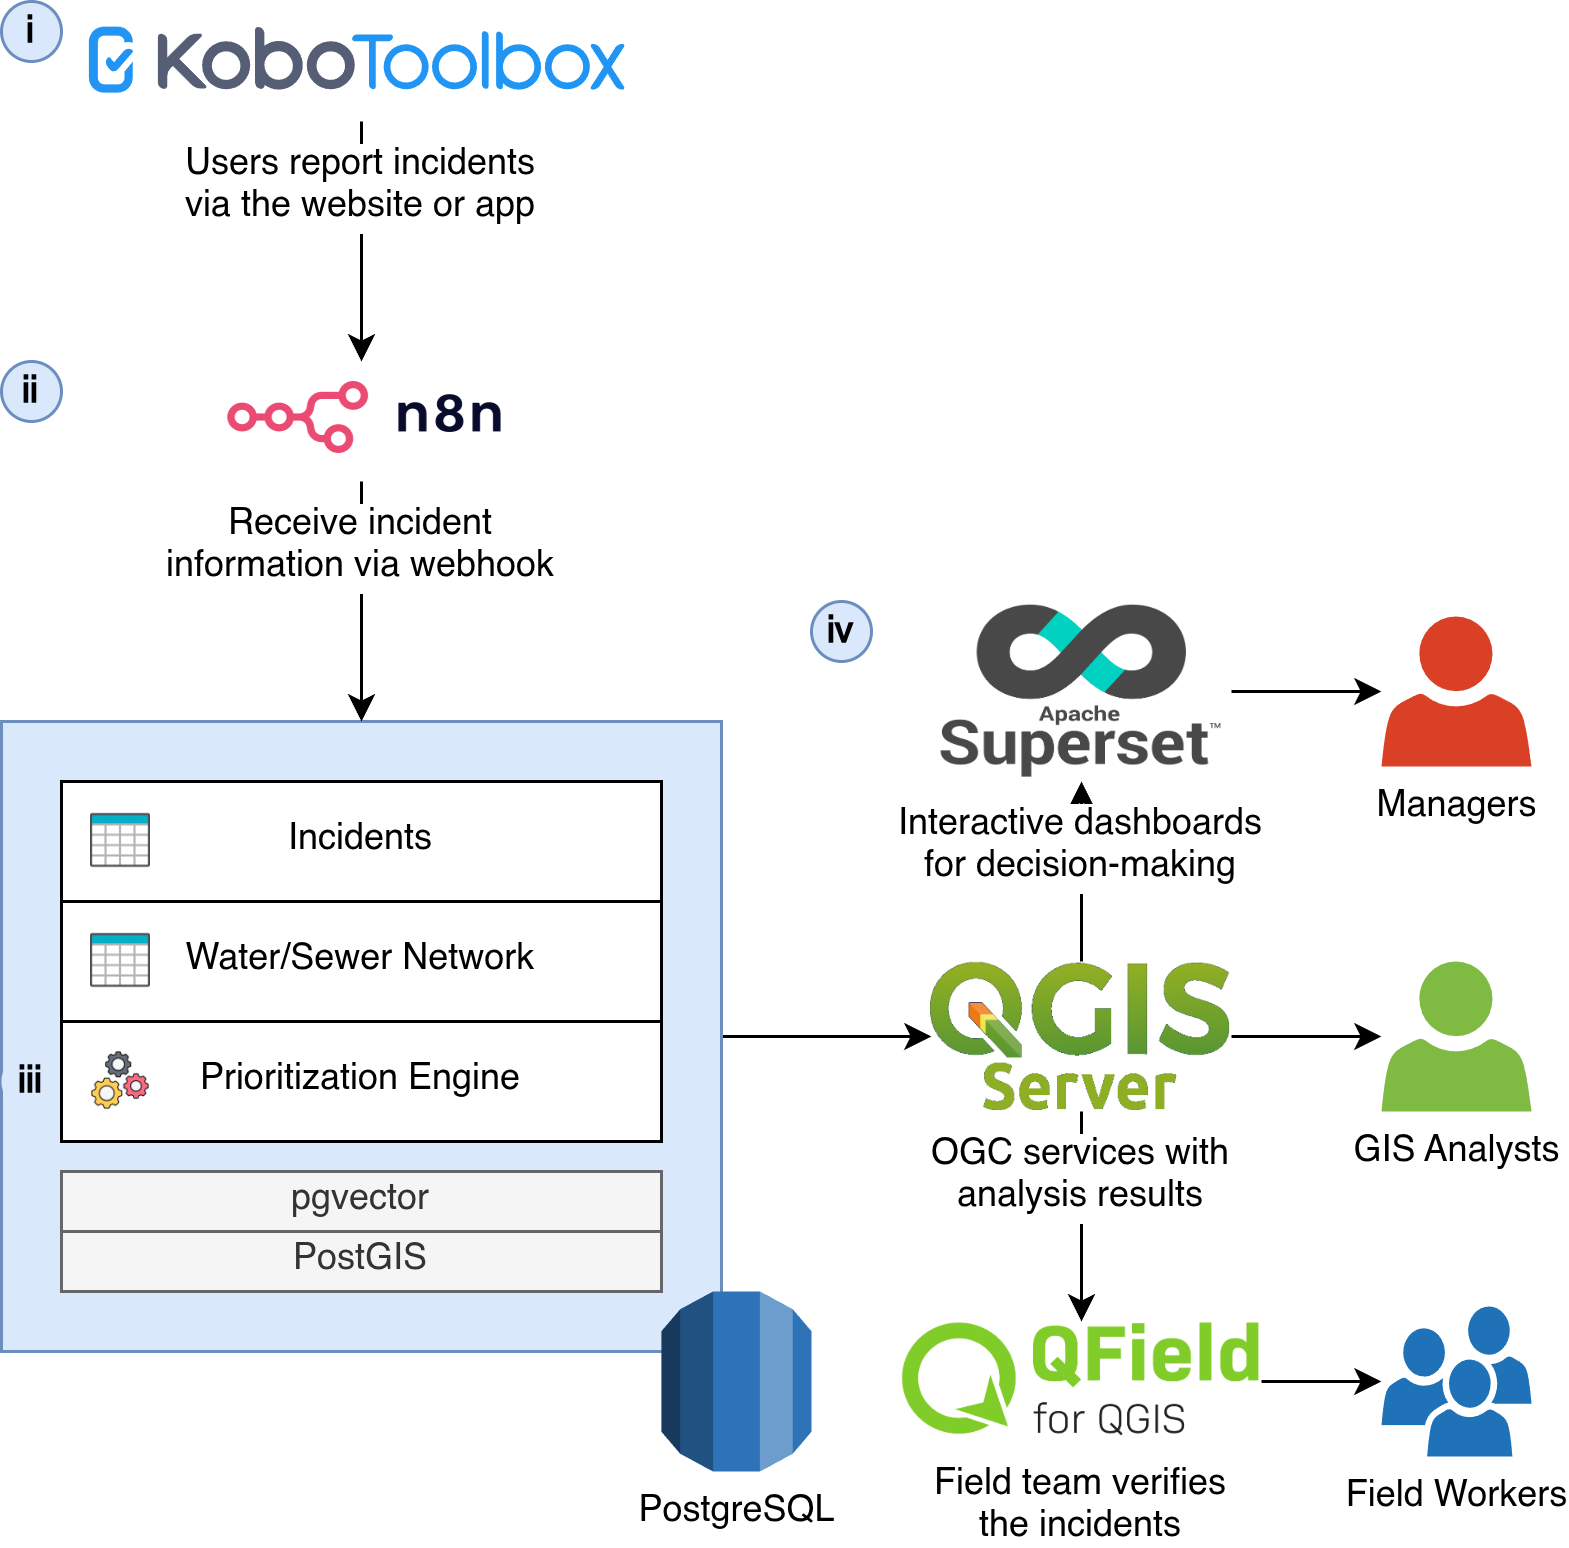
\includegraphics[width=\columnwidth]{assets/architecture.png}
    \caption{System architecture diagram showing the event-driven flow from VGI collection to decision support.}
    \label{fig:architecture}
\end{figure}

\subsection{VGI Collection and Event-Driven Ingestion}

The data acquisition layer is designed to ensure accessibility and operational continuity, utilizing KoboToolbox as the primary interface for field data collection. KoboToolbox provides an ODK-compliant (Open Data Kit) environment that allows for the creation of geospatially enabled forms capable of capturing point geometries, timestamps, photographic evidence, and descriptive metadata regarding water incidents. This choice is strategic for small entities and NGOs, as it offers an offline-first capability; reports generated in areas with poor connectivity are cached locally on the device and automatically transmitted once a network connection is established, preventing data loss in remote or underserved regions \cite{brovelli2016, mcdonald2025}.

The integration between the collection front-end and the spatial database is managed through an event-driven architecture orchestrated by n8n. Instead of traditional polling mechanisms, the proposed workflow relies on webhooks to trigger immediate data ingestion. Upon form submission, the orchestrator receives the information via JSON through the webhook call, storing the spatial and alphanumeric data, along with references to potential attachments via URLs, directly into the database. Finally, the orchestrator initiates the incident prioritization process within the database, considering the newly inserted occurrence.

\subsection{In-Database Spatial Prioritization Algorithm}

The core analytical engine of the proposed architecture resides within the Spatial Database Management System (SDBMS). Once raw VGI data is ingested into PostgreSQL/PostGIS, an automated spatial prioritization algorithm is triggered via internal stored procedures. This native execution leverages the robust indexing and computational efficiency of PostGIS, avoiding the latency typically associated with transferring large geometries to external middleware or desktop GIS environments \cite{obe2021}. The algorithm comprises two sequential mathematical operations: spatial redundancy resolution and multi-criteria urgency scoring.

The first step addresses the inherent redundancy of crowdsourced data. High-impact water incidents often generate multiple citizen reports within a short time frame and localized geographic area. To consolidate these duplicate inputs, the algorithm employs a spatial clustering technique using the native \texttt{ST\_ClusterDBSCAN} function. Instead of relying strictly on traditional Euclidean measurements, the spatial evaluation parameter is modeled around the Minkowski distance metric. As demonstrated by recent literature \cite{haviluddin2020, karo2025}, utilizing Minkowski-based spatial assessments in clustering algorithms provides superior adaptability for urban networks. The Minkowski distance between two points, $X$ and $Y$, in an $n$-dimensional space is defined as:

\begin{equation}
    D(X, Y) = \left( \sum_{i=1}^{n} |x_i - y_i|^p \right)^{1/p}
    \label{eq:minkowski}
\end{equation}

A critical factor in the effectiveness of this clustering stage is the selection of the \textit{epsilon} ($\epsilon$) parameter, which defines the maximum distance for a point to be considered in the neighborhood of another. The choice of $\epsilon$ is highly sensitive and directly impacts the granularity of the identified clusters \cite{rahmah2020}. Given the dynamic nature of urban VGI, the automatic tuning of this parameter is essential to maintain high clustering accuracy across different population densities \cite{starczewski2020}. In this study, the methodology for generating organic synthetic incidents, detailed in Subsection \ref{sub:demographic-driven-synthetic-incident-generation}, serves as a controlled environment for the calibration and benchmarking of the optimal $\epsilon$ value, ensuring it reflects realistic urban reporting patterns.

Once the \texttt{ST\_ClusterDBSCAN} function assigns a cluster ID based on the calibrated $\epsilon$ and the Minkowski metric, the system utilizes the \texttt{ST\_Collect} function. This step geometrically aggregates the grouped points into a single MultiPoint object, from which a centroid is extracted to materialize the unified "Incident Node" \cite{dealbuquerque2015}. This prevents the operational dashboard from being overwhelmed by duplicate notifications.

Following consolidation, the algorithm computes an Urgency Score for each Incident Node using a spatial Multi-Criteria Decision Analysis (MCDA) approach \cite{zyoud2016}. The scoring procedure calculates proximity metrics between the node and critical infrastructure layers (e.g., hospitals, schools), along with pipe diameter and population density weights, allowing for an objective triage of interventions.

\subsection{Demographic-Driven Synthetic Incident Generation} \label{sub:demographic-driven-synthetic-incident-generation}

To address the "cold start" challenge and overcome the inaccuracies of uniform random generation \cite{mcalinden2024}, this study implements a census-weighted simulation model within the SDBMS. The methodology utilizes high-resolution demographic data, including the number of inhabitants and households per census tract, integrated with building footprints retrieved from the Google Open Buildings dataset \cite{sirko2021}. By intersecting these layers, the system calculates a weighted probability surface where reporting frequency is proportional to population density. Furthermore, the model simulates realistic data redundancy by generating repeated reports at roughly the same coordinates for high-density structures, such as condominiums, based on their estimated occupancy.

In the final step of the pipeline, the spatial positioning of these synthetic incidents follows a stochastic translation. To ensure a uniform distribution within a search radius ($D_{max}$), the algorithm implements a polar-to-cartesian transformation. For any given network point, the coordinates of a synthetic incident $(X, Y)$ are computed as follows:

\begin{equation}
    \begin{cases} 
    X = X_{node} + \cos(2\pi \cdot r_1) \cdot (\sqrt{r_2} \cdot D_{max}) \\
    Y = Y_{node} + \sin(2\pi \cdot r_1) \cdot (\sqrt{r_2} \cdot D_{max})
    \end{cases}
    \label{eq:translation}
\end{equation}

where $r_1$ and $r_2$ are independent random variables $\in [0, 1)$. This geometric logic, executed via PL/pgSQL stored procedures, not only enables the generation of behaviorally accurate urban hotspots but also introduces a stochastic variability that accurately simulates the inherent lack of precision typical of smartphone indoor positioning systems \cite{liu2025}. These realistically scattered clusters serve as the ground truth for stress-testing the n8n ingestion pipeline and calibrating the \textit{epsilon} ($\epsilon$) and \textit{minpoints} parameters of the \texttt{ST\_ClusterDBSCAN} function, ensuring the system can effectively distinguish between localized network failures and genuinely redundant citizen reports \cite{starczewski2020}.

\subsection{Open Data, Interoperability, and Humanitarian Integration}

To maximize the societal impact of the collected VGI, the dissemination layer is built exclusively upon open data paradigms and interoperability standards. QGIS Server is deployed to expose the prioritized incident clusters via Open Geospatial Consortium (OGC) protocols, specifically Web Map Service (WMS) and Web Feature Service (WFS). This guarantees seamless technical interoperability with external Geographic Information Systems, enabling the fluid exchange of geospatial information without proprietary barriers \cite{coetzee2020review}. Furthermore, the architecture implements automated data pipelines to publish the processed incidents into global humanitarian repositories, such as the Humanitarian Data Exchange (HDX), and national open data portals. Sharing structured, real-time civic data not only supports immediate infrastructure relief efforts but also serves as a foundational condition for the development of smart city ecosystems and sustainable urban applications \cite{seljan2022}.

\section{Results and Discussion}

The proposed architecture was evaluated using geospatial data from the Metropolitan Region of Vitória, Espírito Santo, Brazil. This study area was selected due to the high quality and precision of the state's open data platform, GEOBASES \cite{geobases_ide}, which provided the complete water distribution and adduction network, along with associated operational assets. Figure \ref{fig:study_area} illustrates the study area and the spatial distribution of the utility network used as the backbone for the simulations.

\begin{figure}[ht]
    \centering
    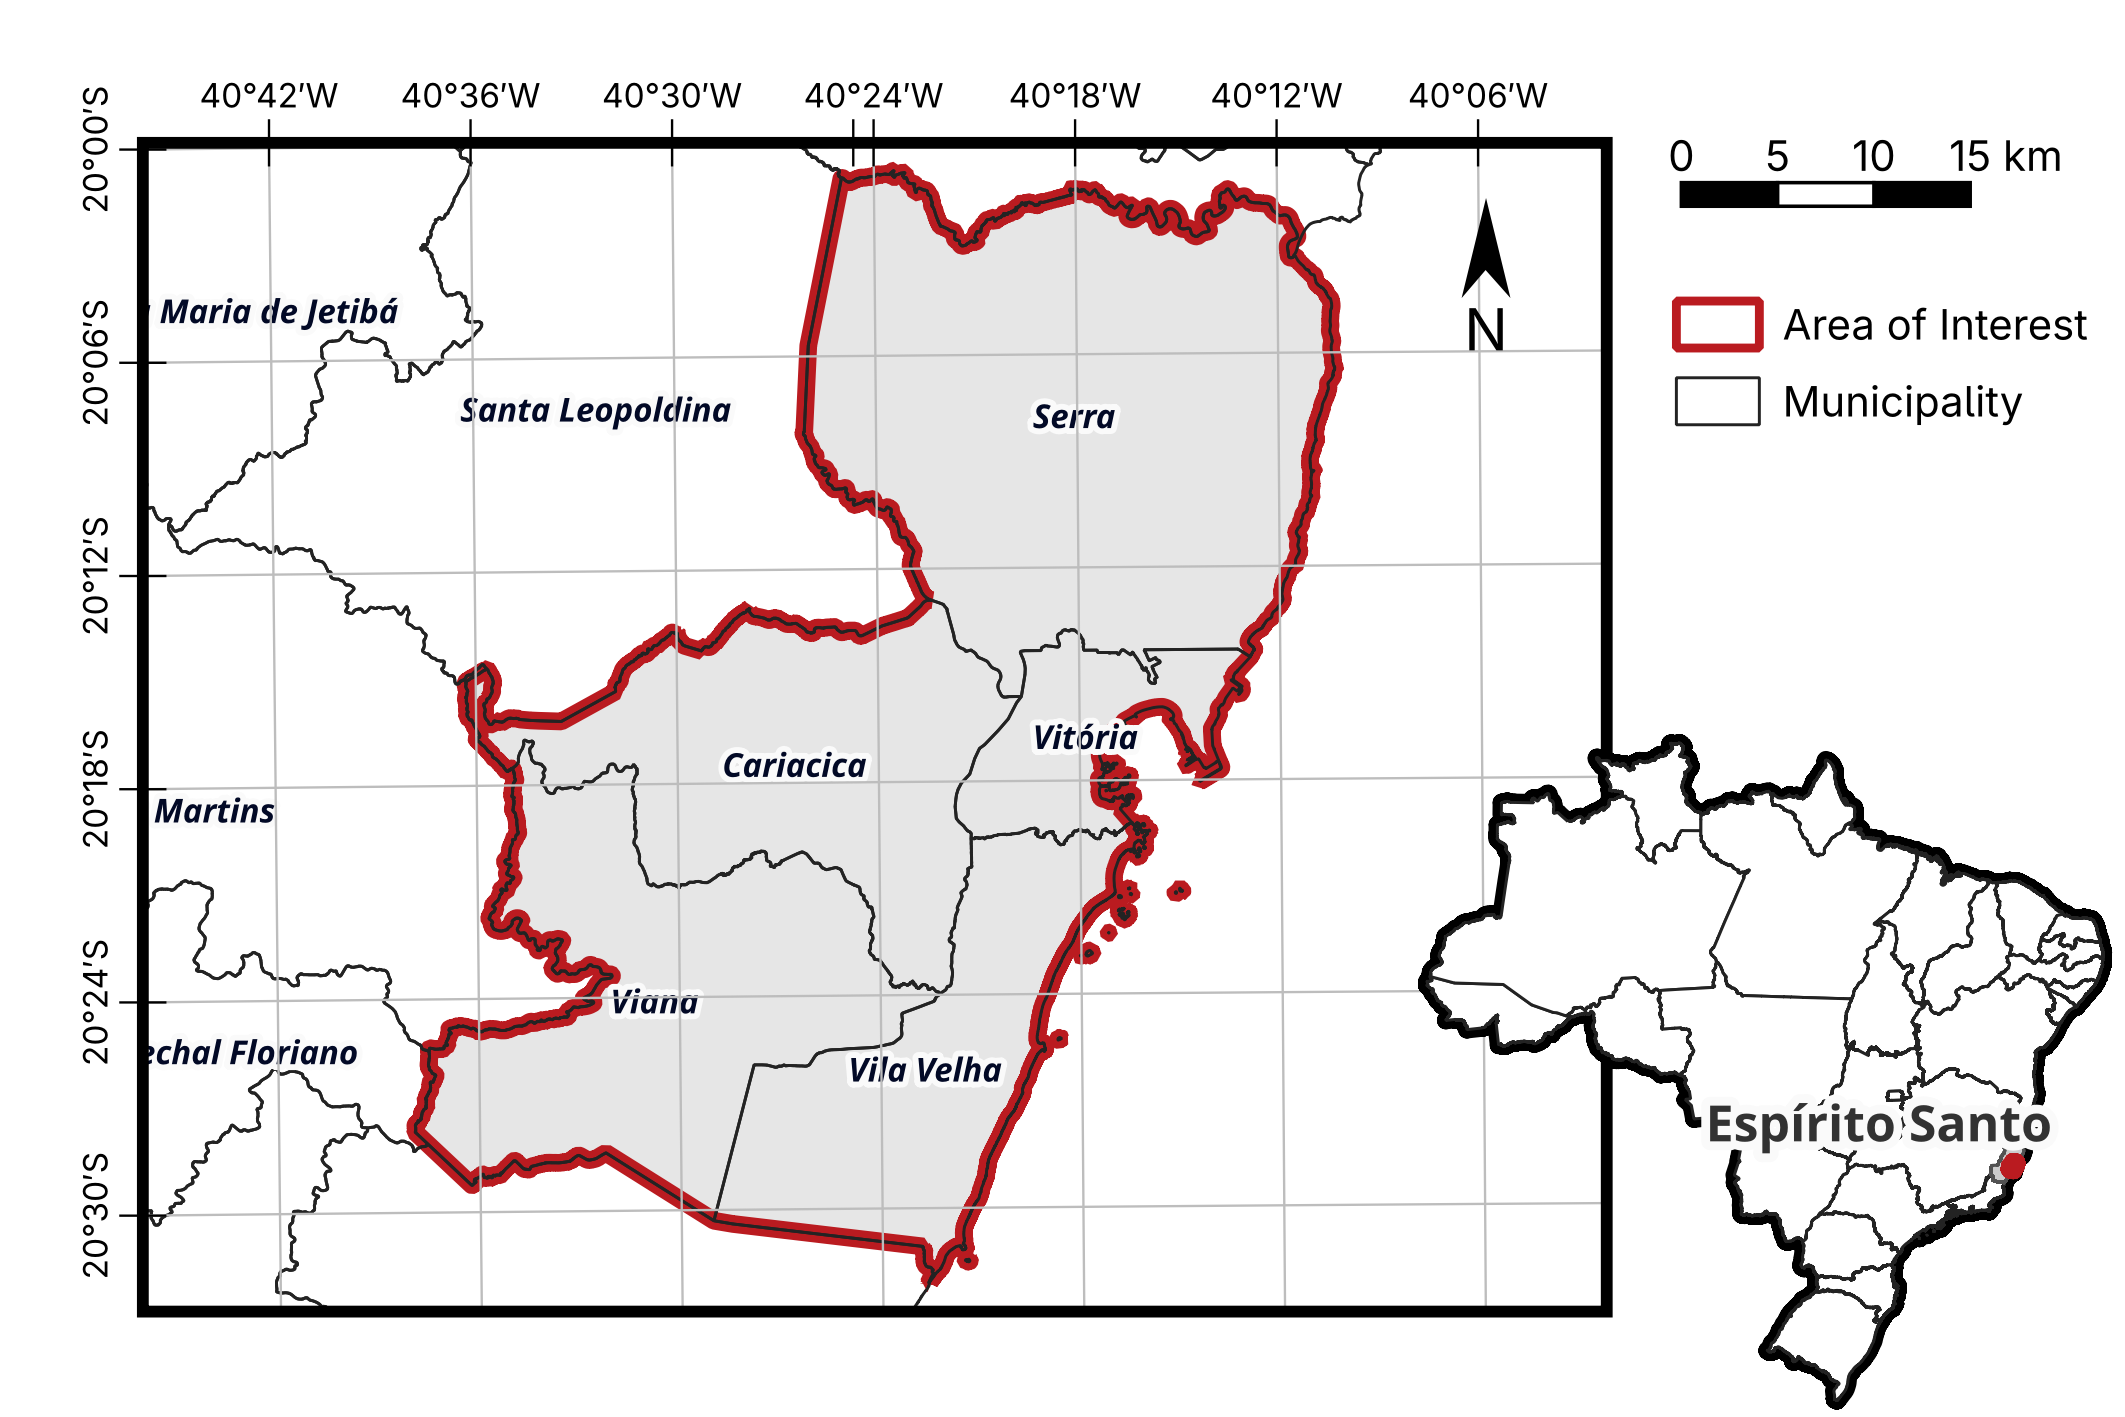
\includegraphics[width=\columnwidth]{assets/aoi.png}
    \caption{Map of the area of interest: the Metropolitan Region of Vitória, Espírito Santo, Brazil; in red.}
    \label{fig:study_area}
\end{figure}

By applying the demographic-driven generation model (Subsection \ref{sub:demographic-driven-synthetic-incident-generation}) over the network, it was possible to simulate 1,000 incident reports in a 72 hours interval, statistically distributed over the service territory according to the proposed model. The calibration of the \textit{epsilon} parameter ($\epsilon$) at 400 meters, using the Minkowski distance ($p=1.5$) to reflect the local urban morphology. The \textit{epsilon} parameter ($\epsilon$) were also tunned to represent the median distance between a given consumer and its nearest reservoir, pumping station or treatment plant.

The DBSCAN algorithm, executed natively in PostGIS, successfully consolidated redundant reports into unique Incident Nodes with a reduction rate of 72\% in total active notifications, significantly decreasing the visual noise for humanitarian operators without omitting critical failures. As exposed by Figure \ref{fig:comparison}.

\begin{figure}[ht]
    \centering
    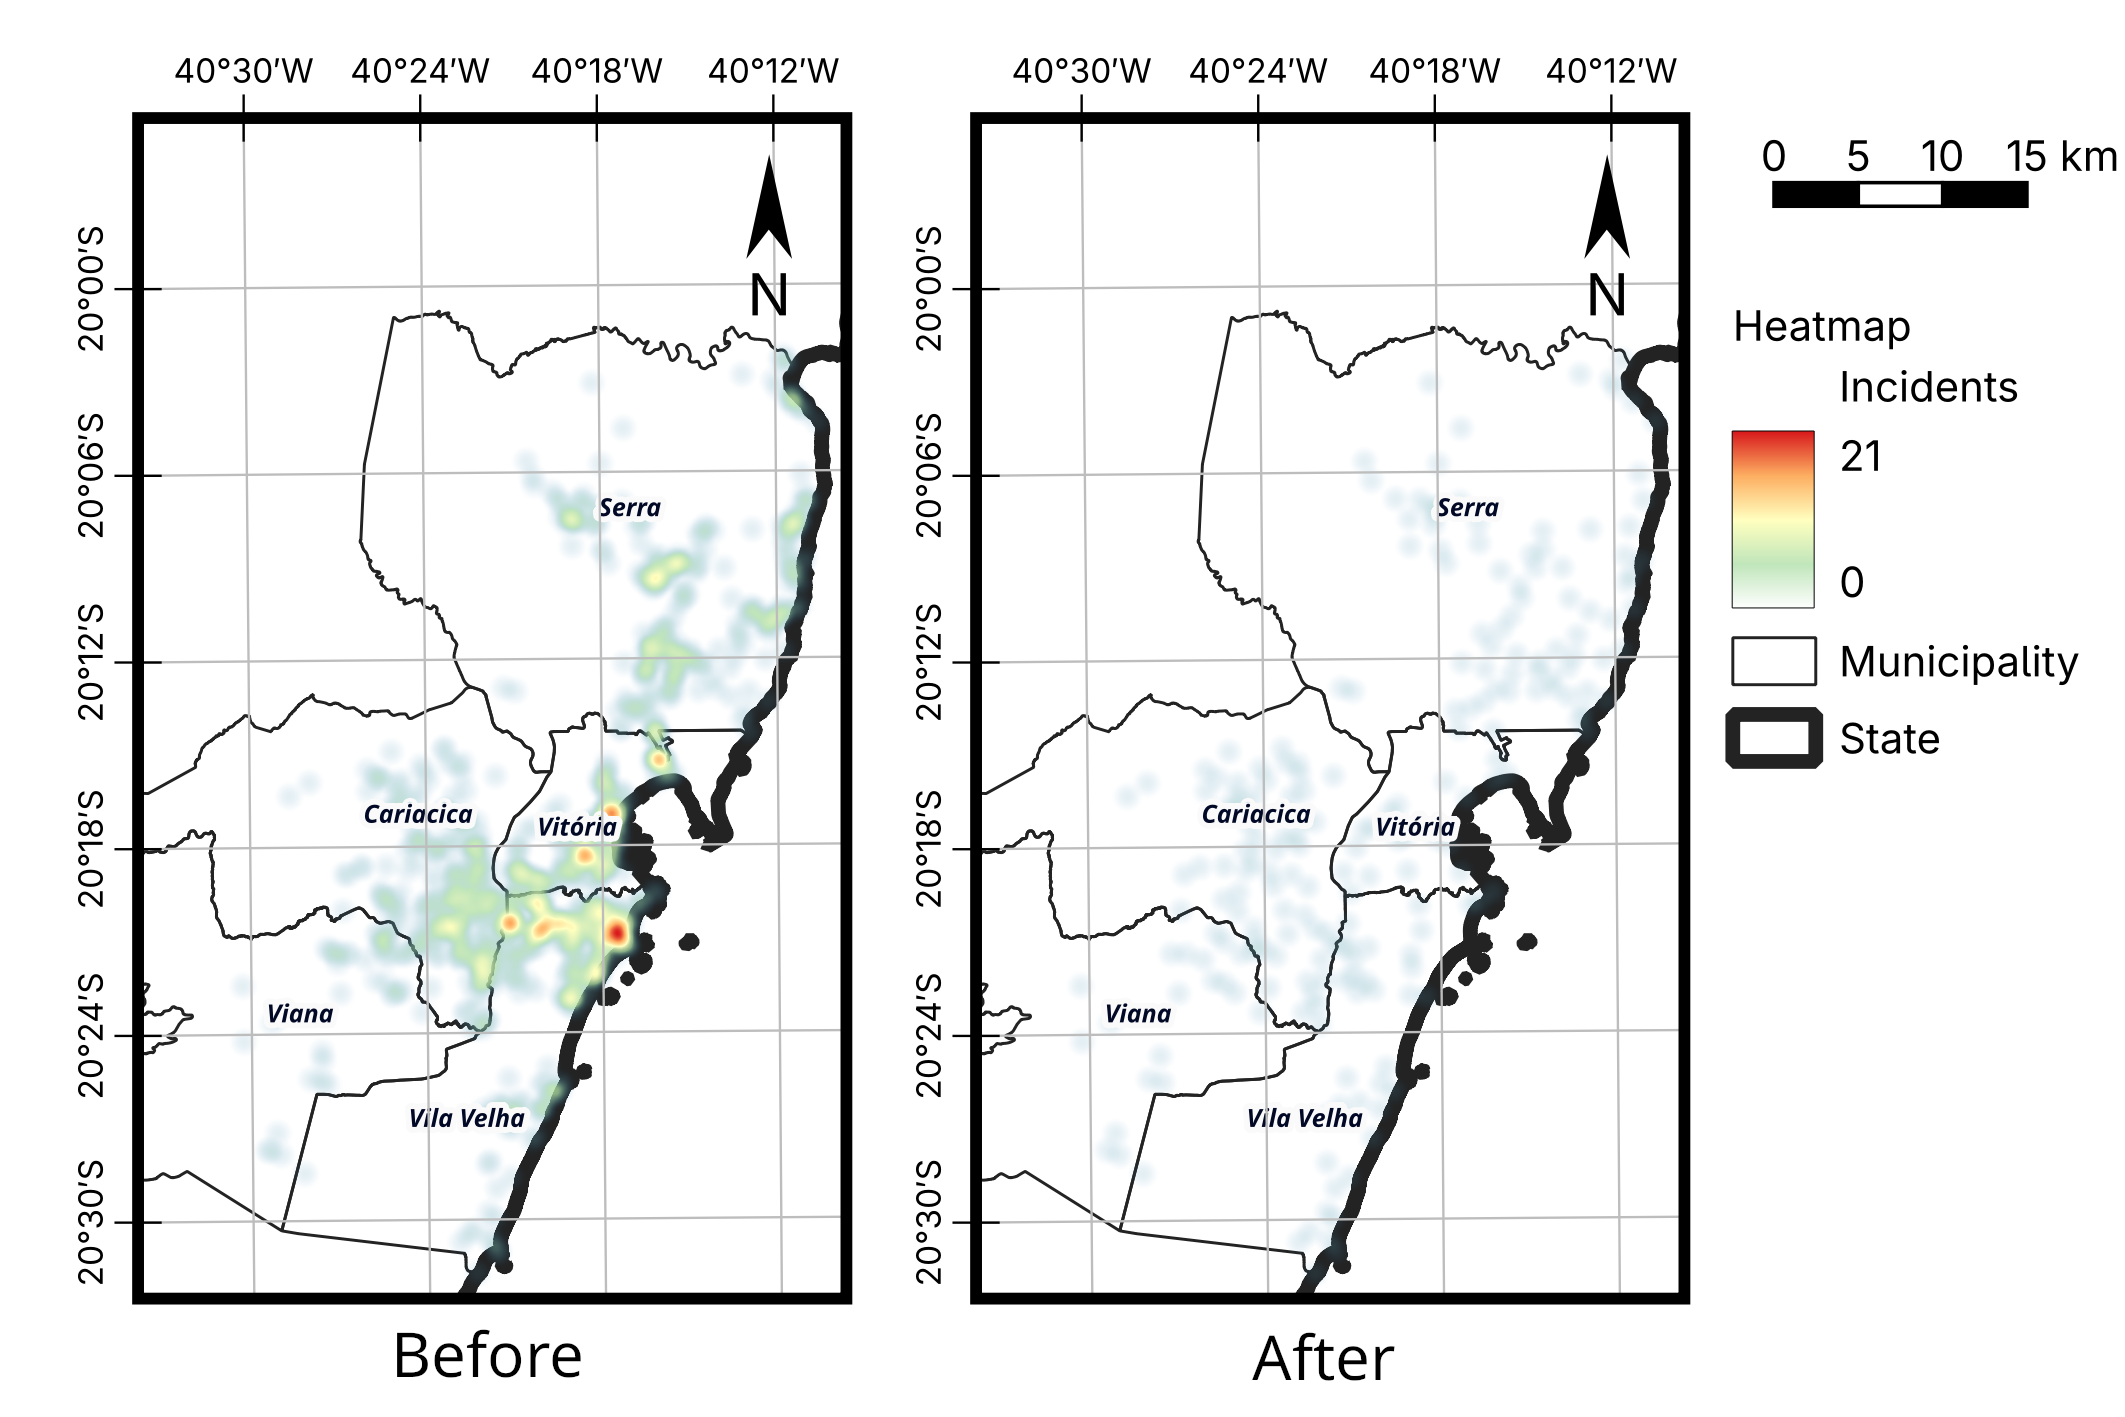
\includegraphics[width=\columnwidth]{assets/comparison.png}
    \caption{Comparison of the total number of occurrences before (left) and after (right) clustering.}
    \label{fig:comparison}
\end{figure}

The application of the spatial Multi-Criteria Decision Analysis (MCDA) fundamentally reordered the maintenance queue compared to a standard First-In-First-Out (FIFO) approach. In the simulated scenarios, incidents occurring within a 200-meter radius of essential health facilities in Vitória were automatically elevated to maximum priority. For instance, a major leak reported near a regional hospital was repositioned from the 38th to the 1st rank in the intervention matrix immediately upon ingestion. This real-time re-prioritization demonstrates the system's ability to transform raw citizen-generated data into actionable, high-impact humanitarian intelligence, ensuring that limited maintenance resources are allocated where they are most urgently needed to maintain public health and service continuity.

\section{Conclusion}

This paper presented a 100\% open-source, event-driven architecture for monitoring water distribution incidents through Volunteered Geographic Information (VGI). By decoupling data collection via KoboToolbox from a high-performance analytical engine in PostGIS, the system effectively addresses the dual challenge of low-cost infrastructure and real-time spatial processing. The methodology introduced a demographic-driven synthetic generation model, which proved essential for calibrating spatial clustering parameters—specifically the \textit{epsilon} in DBSCAN—simulating realistic urban reporting patterns and indoor positioning noise.

Validation using real-world network data from the Metropolitan Region of Vitória (GEOBASES) demonstrated a 72\% reduction in redundant notifications through in-database spatial consolidation. Moreover, the integration of spatial Multi-Criteria Decision Analysis (MCDA) enabled a prioritized humanitarian response, successfully reallocating critical incidents near essential services to the top of the intervention queue. Future work will explore the integration of GeoAI models for automated image validation and the expansion of this framework to other urban infrastructure domains. This study concludes that an SDBMS-centric, open-source approach provides a scalable and interoperable foundation for smart city management and humanitarian relief efforts.

\section*{Code Availability}
To ensure reproducibility and foster community collaboration, the complete artifacts developed for this study are publicly accessible at \url{https://github.com/teofilosalgado/eu-salvo-agua}. The repository provides the native source code for the spatial clustering, prioritization, and synthetic data generation mechanisms, alongside the Kubernetes YAML manifests required to automatically deploy the entire application ecosystem.

\bibliographystyle{IEEEtran}
\bibliography{IEEEabrv,main}

\end{document}
